\documentclass[12pt]{article}

\usepackage{fullpage}
\usepackage{multicol,multirow}
\usepackage{tabularx}
\usepackage{listings}
\usepackage[utf8]{inputenc}
\usepackage[russian]{babel}
\usepackage{graphicx}
\usepackage{csquotes}

\begin{document}

\begin{titlepage}

    \begin{center}

        \bfseries
        {\small Московский авиационный институт\\ 
        (национальный исследовательский университет)}

        % \vspace{48pt}
        {\small Факультет информационных технологий и прикладной 
        математики}
        
        % \vspace{36pt}
        {\small Кафедра вычислительной математики и программирования}
        
        \vspace{8cm}
        {\Large Лабораторная работа \textnumero 6 по курсу} 
        \enquote{\Large Компьютерная графика}
        
    \end{center}
    
    \vspace{84pt}
    \begin{flushright}
        \begin{tabular}{rl}
            Студент: & Е.Ю. Юрков \\
            % Преподаватель: &  \\
            Группа: & М80-312Б-22 \\
            Дата: & \\
            Оценка: & \\
            Подпись: & \\
        \end{tabular}
    \end{flushright}
    
    \vfill
    
    \begin{center}
        
        \bfseries
        Москва, \the\year
    
    \end{center}

\end{titlepage}

% Выполнил студент группы М8О-312Б-22 МАИ \textit{Юрков Евгений}.

\subsection*{Цель лабораторной работы}

Цель лабораторной работы:
В этой лабораторной работе вы будете разрабатывать основу для собственного игрового
движка. Это завершающая работа, в которой вы объедините все изученные техники работы
с 2D и 3D графикой, освещением, шейдерами и трассировкой лучей. В результате
выполнения лабораторной работы у вас должен получиться простой движок, который
может отрисовывать сцены в реальном времени, с возможностью работы с камерой,
объектами и освещением.
Основные задачи:
\begin{enumerate}
    \item Создать базовую архитектуру игрового движка с поддержкой 3D-сцен.
    \item Реализовать систему рендеринга с использованием изученных подходов: рендеринг через растризацию и трассировку лучей.
    \item Настроить камеру и систему управления ею.
    \item Реализовать поддержку базовых игровых объектов и взаимодействие с ними.
    \item Обеспечить работу с несколькими типами источников света.
    \item Оптимизировать производительность движка (по возможности).
\end{enumerate}

% \newpage
\subsection*{Метод решения}

Движок я решил реализовать в качестве библиотеки. Она имеет следующую структуру:
\begin{itemize}
    \item camera - директория, содержащая классы для работы с камерой, а именно для отправления матрицы камеры в шейдер.
        \begin{itemize}
            \item Camera.hpp - основной класс для работы с камерой. Позволяет задавать позицию камеры и позицию цели камеры.
            Также в этом файле содержится структура, позволяющая задавать настройки камеры, например, проекцию, плоскости отсечения, угол обзора.
            \item FPCamera.hpp - класс для камеры от первого лица, наследует класс Camera, а также имеет методы для обработки мыши и привязки к объекту.
            \item TPCamera.hpp - класс для камеры от третьего лица, наследует класс Camera, а также имеет методы для обработки мыши и привязки к объекту.
        \end{itemize}
    \item objects - директория, содержащая классы основных объектов и класс модели (.obj).
        \begin{itemize}
            \item ObjectBase.hpp - базовый класс для всех фигур, задаёт интерфейс взаимодействия с объектами, а также определяет операции
            для перемещения объектов через матрицу модели.
            \item Cube.hpp - класс куба, позволяет также накладывать текстуру на куб.
            \item Flat.hpp - класс плоскости, с текстурой.
            \item Model.hpp - класс для обработки фигуры из файла .obj, берёт текстуру для модели из файлов указанных в файле .mtl.
        \end{itemize}
    \item shader - директория, содержащая класс Shader для удобной компиляции шейдеров и работы с ними.
    \item texture - директория, содержащая класс Texture для установки текстур и работы с ними.
    \item light - директория, содержащая классы источников света.
        \begin{itemize}
            \item PointLight.hpp - класс точечного источника света, позволяет установить цвет освещения.
            В шейдере учитывается расстояние от источника для затухания.
            \item DirectLight.hpp - класс направленного света.
        \end{itemize}
    \item logic - директория, содержащая классы событий, которые обрабатывает движок.
        \begin{itemize}
            \item Event.hpp - базовая структура события, содержит всего два поля: condition и action - условие, по которому возникает
            событие и действие, которое должно быть совершено. 
            \item FrameEvent.hpp - событие, срабатывающее на каждом кадре.
            \item EveryNSec.hpp - событие, срабатывающее каждые N секунд.
            \item KeyboardEvent.hpp - событие, срабатывающее при нажатии определённой кнопки.
            \item MouseEvent.hpp - событие, срабатывающее при движении мыши, action для этого события должен принимать offsetx, offsety и scroll.
            \item IntersectEvent.hpp - событие, проверяющее пересечение bounding box объектов.
        \end{itemize}
    \item engine - директория, содержащая основной класс движка - сцену.
        \begin{itemize}
            \item Scene.hpp - класс сцены. Позволяет привязывать к сцене объекты, источники света, камеру и назначать события.
        \end{itemize}
\end{itemize}

В итоге на разработанном движке была создана игра, где снеговик, перемещаясь по ограниченному полю, 
должен был ловить снежинки и вырасти благодаря им до определённого размера.

\subsection*{Результат работы программы}

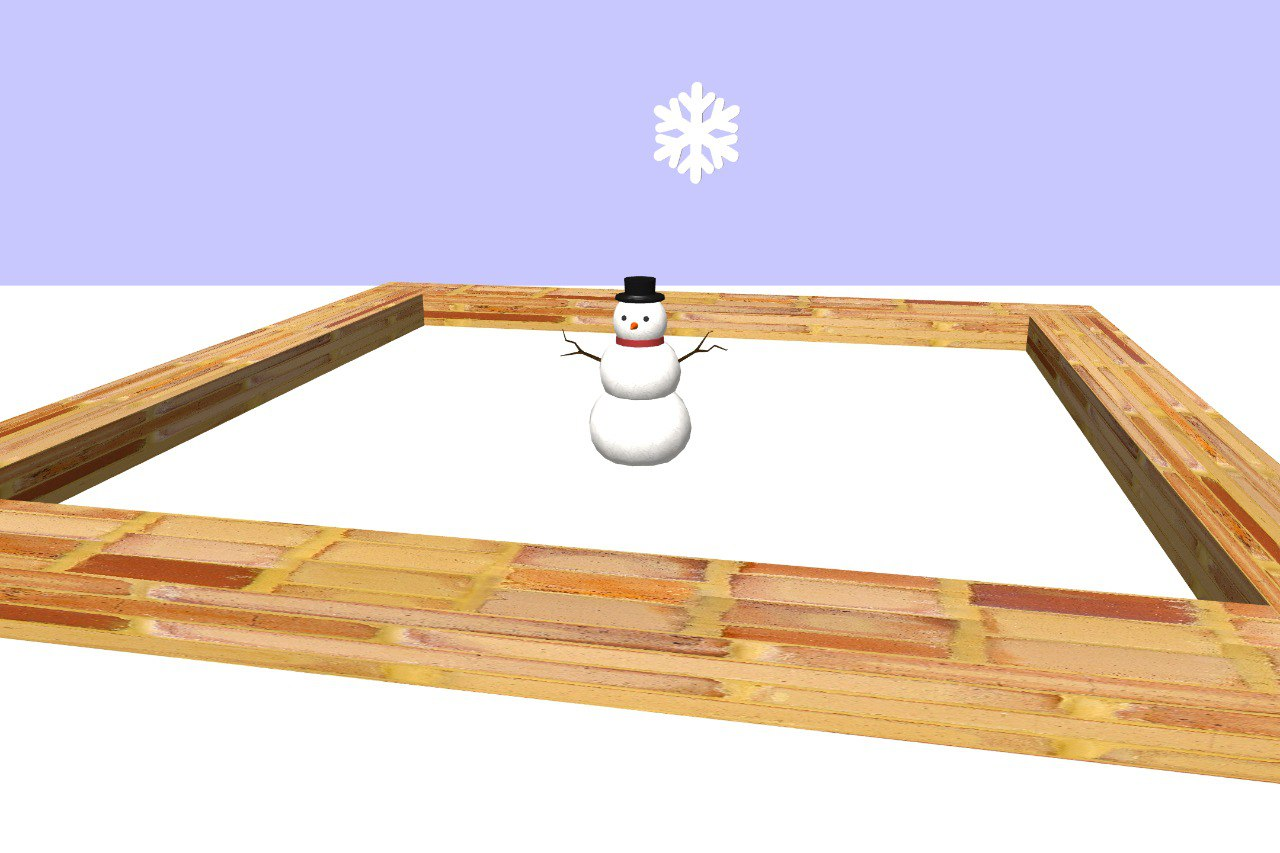
\includegraphics[width=15cm]{demo.jpg}

% \newpage
\subsection*{Выводы}

В ходе выполнения этой лабораторной работы я укрепил знания, полученные в курсе компьютерной графики.
Я изучил устройство и структуру obj файлов, а также написал класс для загрузки объектов из файла.
Также эта лабораторная позволила углубить знания в области разработки игр.

\end{document}